\chapter{相关技术介绍}\label{chap:introduction}

由于本硬件加速系统设包含了软件与硬件的协同设计,所以本章将对涉及到的关键技术,包括深度神经网络算法、ZYNQ 器件做基本的介绍。如第一章节所述,本章还会对不同类型的硬件加速体系结构进行基本概述,介绍对应的应用案例。


\section{深度神经网络概述}

\subsection{单层感知机模型}

\begin{figure}[!htbp]
    \centering
    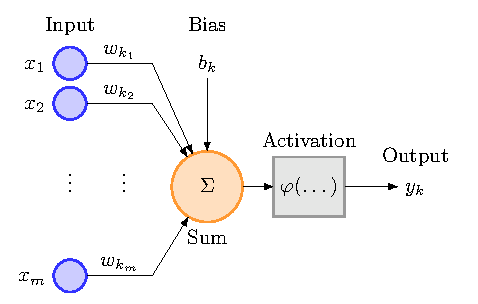
\includegraphics[width=0.5\textwidth]{neuron}
    \caption{神经元模型}
    \label{fig:neuron}
\end{figure}

一个神经元的模型如图~\ref{fig:neuron}所示,该模型也被称为单层感知机,由输入信号、权值、偏置、加法器和激活函数共同构成,其中 $w_{kj}$ 下标的含义为:$k$ 表示第 $k$ 个神经元;$j$ 表示第 $j$ 个输入。因此,$w_{kj}$表示第 $k$ 个神经元的第 $j$ 个输入对应的权值。单个神经元的数学公式如公式~\eqref{eq:neuron} 所示:

\begin{equation} \label{eq:neuron}
% \adddotsbeforeeqnnum%
\begin{cases}
u_k = \sum_{j=1}^{m} w_{kj}x_j & \\
v_k = u_k + b_k & \\
y_k = \varphi(v_k) &
\end{cases}
\end{equation}

其中 $x_j$ 表示第 $k$ 个神经元的第 $j$ 个输入,$w_{kj}$表示第 $k$ 个神经元的第 $j$ 个输入对应的权值,$b_k$ 表示第 $k$ 个神经元的偏置,$\varphi(\dots)$ 为激活函数,$y_k$ 为该神经元的输出。

感知器模型于1958年,由美国心理学家Frank Rosenblatt提出,其中激活函数采用的一般是符号函数,如公式~\eqref{eq:sign}所示:

\begin{equation} \label{eq:sign}
    o = sgn(x_1w_1+x_2*w_2+b)
\end{equation}

进一步,为了简化问题分析本质,我们假设神经元只有两个输入: $x_1$ 和 $x_2$ ,则模型的公式进一步简化为:

\begin{equation}
    \begin{cases} 
        1, & x_1w_1+x_2 * w_2+b>=0 \\
        -1, & x_1w_1+x_2*w_2+b<0 
    \end{cases}
\end{equation}

如果把$o$当作因变量、$x_1$ 和 $x_2$当作自变量,对于分界

\begin{equation}
    x_1w_1+x_2w_2+b=0
\end{equation}

可以抽象成三维空间里的一个分割面,能够对该面上下方的点进行分类,则该感知机能完成的任务是用简单的线性分类任务,比如可以完成逻辑“与”与逻辑“或”的分类,如表~\ref{tab:logic}所示,在这里,第三维度只有1和-1两个值,分别使用实心点和空心点来表征,这样就可以在二维平面上将问题可视化:

\begin{table}[!htbp]
    \caption{逻辑 真值表}
    \label{tab:logic}
    \centering
    \footnotesize% fontsize
    \setlength{\tabcolsep}{4pt}% column separation
    \renewcommand{\arraystretch}{1.2}%row space 
    \begin{tabular}{lllllllll}
    \toprule
    \multicolumn{3}{c}{\textbf{逻辑与}}  & \multicolumn{3}{c}{\textbf{逻辑或}} & \multicolumn{3}{c}{\textbf{逻辑异或}}       \\
    $x_1$ & $x_2$ & o & $x_1$ & $x_2$ & o & $x_1$ & $x_2$ & o   \\
    \midrule
    0              & 0              & 0              & 0              & 0              & 0              & 0              & 0              & 0              \\
    0              & 1              & 0              & 0              & 1              & 1              & 0              & 1              & 1              \\
    1              & 0              & 0              & 1              & 0              & 1              & 1              & 0              & 1              \\
    1              & 1              & 1              & 1              & 1              & 1              & 1              & 1              & 0              \\
    \bottomrule
    \end{tabular}
\end{table}

但是对于非线性问题,如异或问题,如图~\ref{fig:Nor}所示,单层感知机没有办法找到一条直线能够完成分类任务。

\begin{figure}[!htbp]
    \centering
    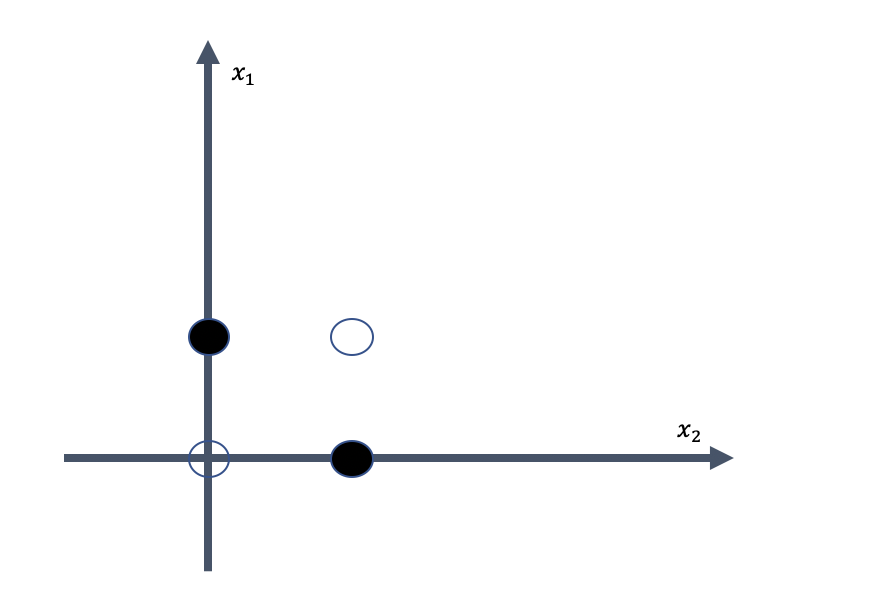
\includegraphics[width=0.6\textwidth]{Nor}
    \caption{异或平面}
    \label{fig:Nor}
\end{figure}

\subsection{多层感知机模型}

多层感知机模型是在单层感知机模型的基础上引入了一层或多层隐藏层,在图~\ref{fig:FNN}所示的多层感知机中,输入和输出的神经元个数分别为4和1,中间的隐藏层包含了5个神经元,隐藏层中的神经元和输入层中各个输入完全连接,输出层中的神经元和隐藏层中的各个神经元也完全连接。因此,多层感知机中的隐藏层和输出层都是全连接层。

\begin{figure}[!htbp]
    \centering
    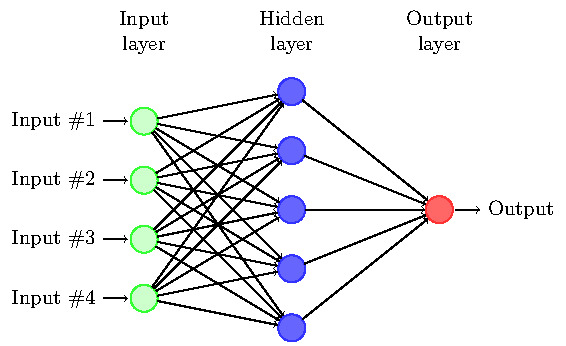
\includegraphics[width=0.6\textwidth]{FNN}
    \caption{前向神经网络结构}
    \label{fig:FNN}
\end{figure}

但是不难发现,即便再添加更多的隐藏层,多层感知机的设计依然只能与仅含输出层的单层神经网络等价。上述问题的根源在于全连接层只是对数据做仿射变换(affine transformation),而多个仿射变换的叠加仍然是一个仿射变换。解决问题的一个方法是引入非线性变换,例如对隐藏变量使用按元素运算的非线性函数进行变换,然后再作为下一个全连接层的输入。这个非线性函数被称为激活函数(activation function),常用的激活函数包括了 Sigmoid、Relu、Tanh 等。

理论上,深度神经网络,及多层感知机已经可以拟合任意的函数\citep{HORNIK1991251}。

\subsection{卷积神经网络概述}

卷积神经网络(Convolutional Neural Network, CNN)是目前最常用的深度神经网络,对于大型图像处理有出色表现,卷积神经网络一般由卷积层、非线性激活函数、池化层组成。

\begin{enumerate}
    \item 卷积层(Convolution Layer)的本质是输入图像与权重矩阵的乘积累加运算(Multiply Accumulate, MAC),如图~\ref{fig:Convolution}所示卷积核在输入特征图像上滑动,用来匹配局部的细节。一般来说,随着卷积的层数逐渐加深,卷积核的数目也会随之增加,所表征的细节也会更加抽象。
    \begin{figure}[!htbp]
        \centering
        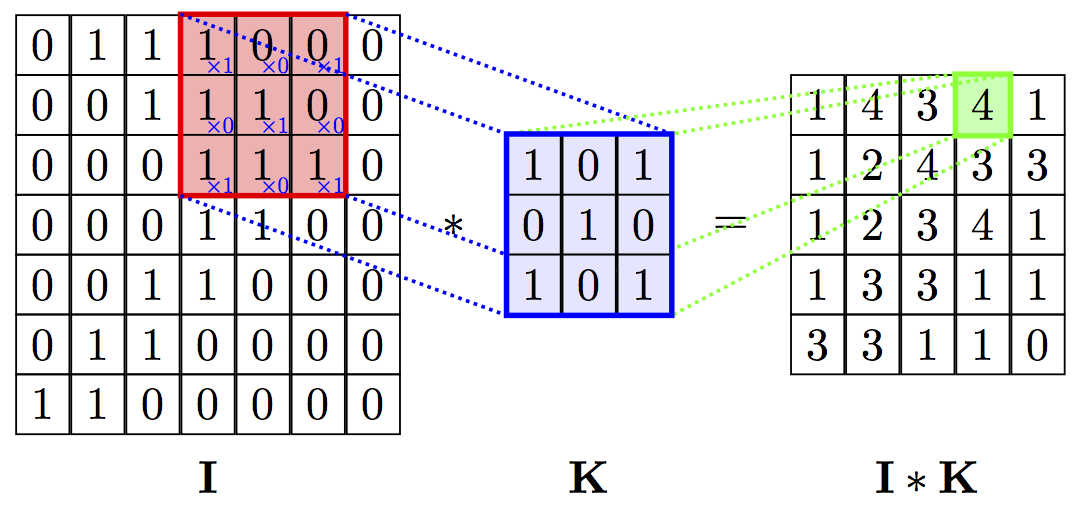
\includegraphics[width=0.6\textwidth]{Convolotion.png}
        \caption{卷积运算}
        \label{fig:Convolution}
    \end{figure}
    \item 激活函数(Activation Function)是非线性单元,它的存在给深度神经网络体系增加了非线性元素,是深度神经网络能够拟合任意函数的基础。比较重要且常用的激活函数有 ReLU、Sigmoid 和 Tanh 。此外,其余常用的激活函数还有 PReLU, ELU 等,他们的函数图像与取值范围如图~\ref{fig:Activation}所示:
    \begin{figure}[!htbp]
        \centering
        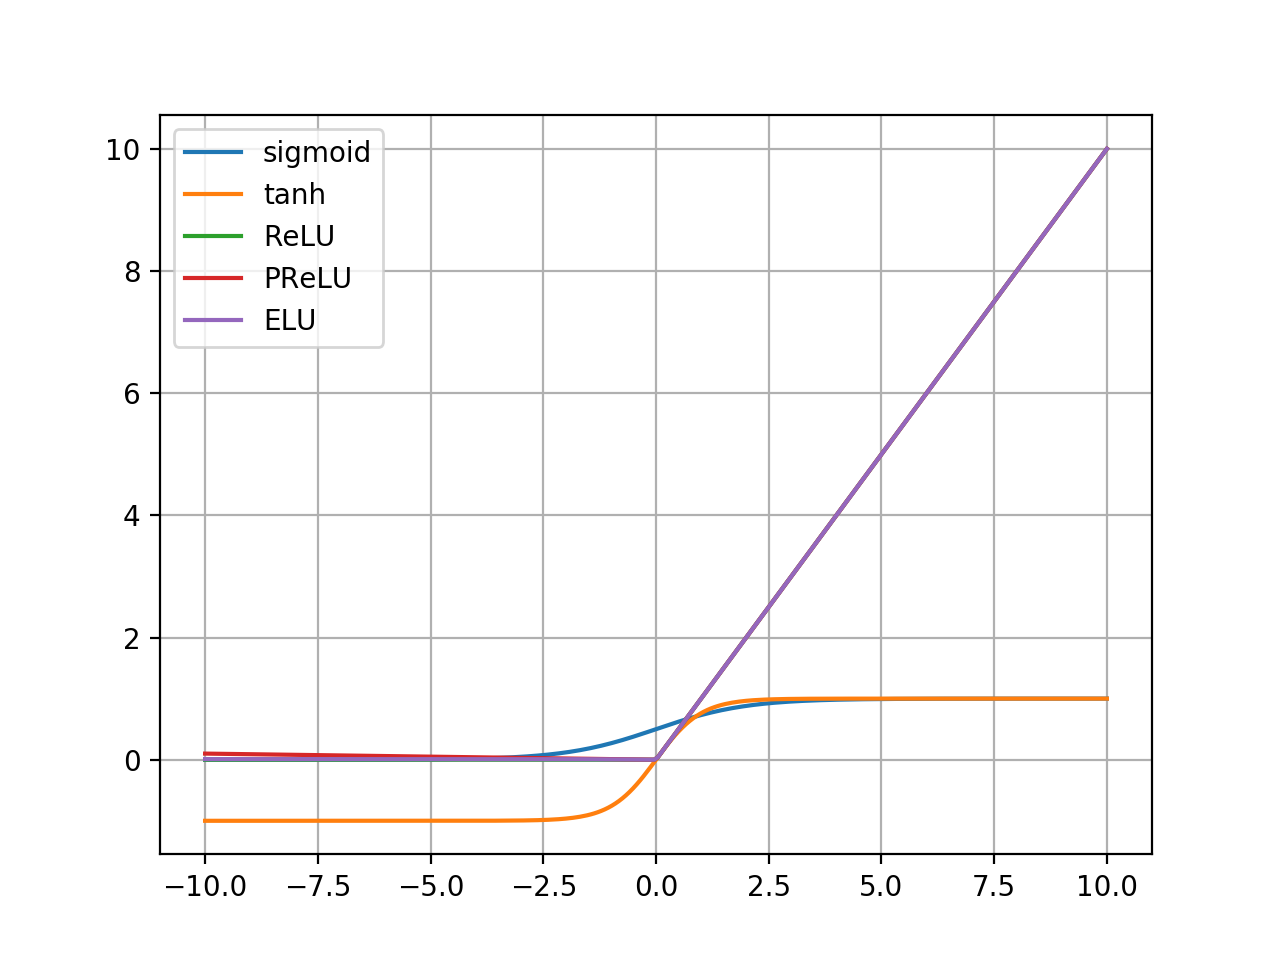
\includegraphics[width=0.6\textwidth]{Activation.png}
        \caption{常见的激活函数图像}
        \label{fig:Activation}
    \end{figure}
    \item 池化层(Pooling Layer)的作用是对特征图进行下采样,从而可以达到增加感受野、增加卷积神经网络运算的平移不变性、降低优化难度,减少神经网络参数的目的。典型的池化层 Max Pooling 如图~\ref{fig:MaxPooling}所示,他会选择被池化矩阵选内最大的值作为输出得到新的特征图。Average Pooling 选取池化矩阵内的平均值,是另一种常用的池化层。
    \begin{figure}[!htbp]
        \centering
        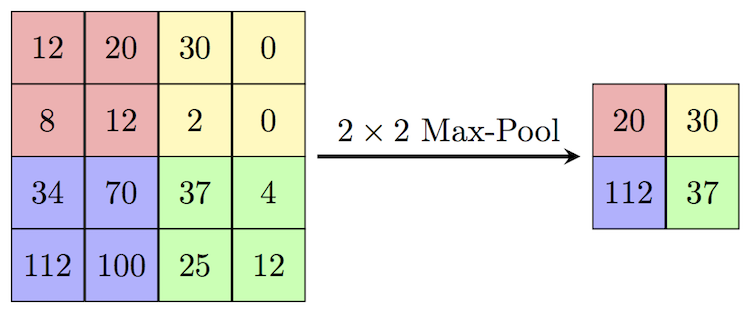
\includegraphics[width=0.6\textwidth]{MaxPooling.png}
        \caption{Max Pooling}
        \label{fig:MaxPooling}
    \end{figure}
\end{enumerate}

\subsection{LeNet5 介绍}

手写字体识别模型LeNet5诞生于1994年,是最早的卷积神经网络之一。

\begin{figure}[!htbp]
    \centering
    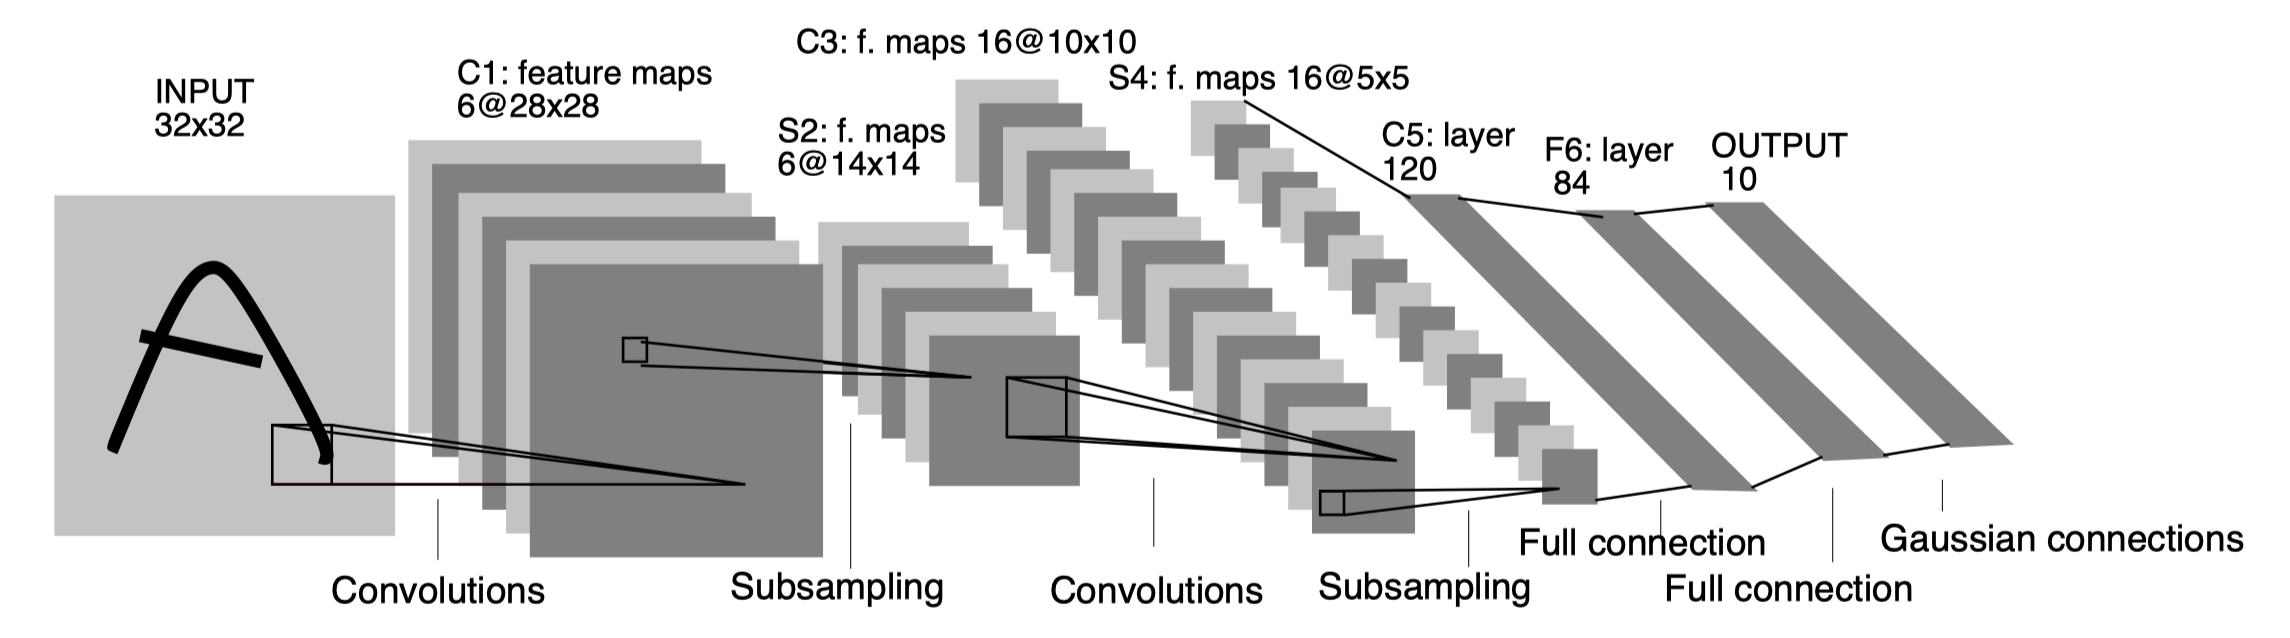
\includegraphics[width=0.9\textwidth]{CNN}
    \caption{LeNet-5 \ 网络结构}
    \label{fig:CNN}
\end{figure}

通过巧妙的设计,利用卷积、参数共享、池化等操作提取特征,LeNet5避免了大量的计算成本,最后再使用全连接神经网络进行分类识别,该网络也是最近大量神经网络架构的起点,LeNet5的网络结构如图~\ref{fig:CNN}所示。

\subsection{Resnet 18 网络结构}

纵观神经网络的发展脉络,我们可以看到研究者一直在不断尝试各种技术以加深神经网络的层数。从8层的 AlexNet,到十九层的 VGG,再到22层的 GoogLeNet,可以说,技术一直在进步。但是在突破神经网络深度的问题上真正最具有颠覆性的技术还是来自 ResNet。

为了避免随着神经网络的深度加深从而带来的退化问题,ResNet 采用了一种不同于常规卷积神经网络的基础结构,其基本单元如图~\ref{fig:Residual}所示,增加了从输入到输出的直连通道。其卷积拟合的是输出与输入的差,及残差,所以这种结构又被称为残差结构。残差网络的响应小于常规网络\citep{DBLP:journals/corr/HeZRS15}。残差网络的优点是对数据波动更加灵敏,更容易求的最优解,能够改善深层网络的训练。

\begin{figure}[!htbp]
    \centering
    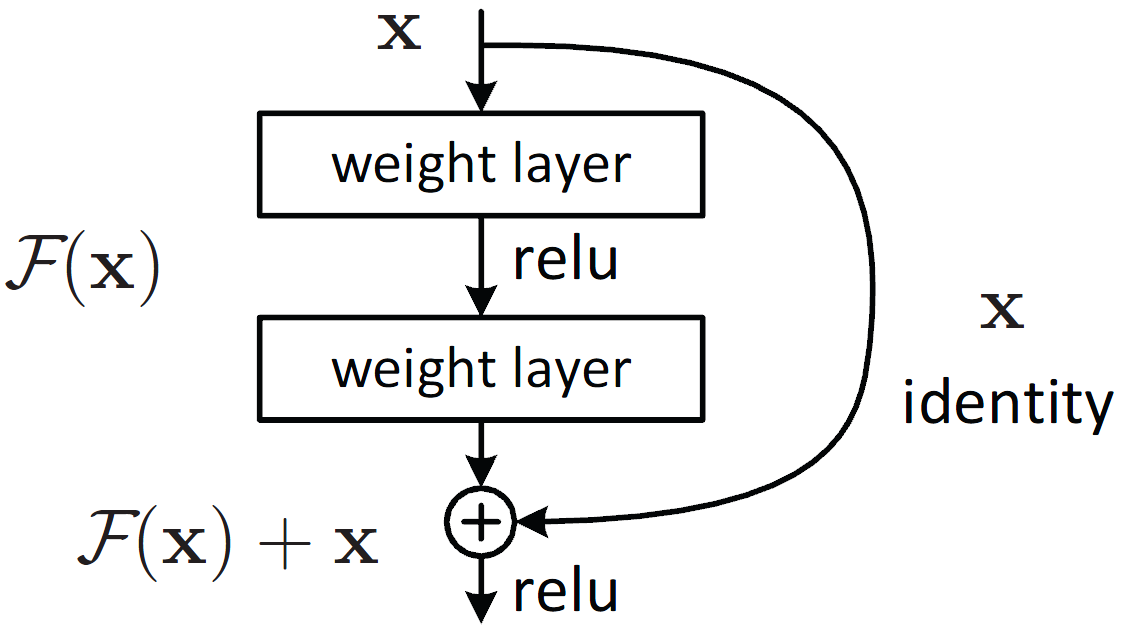
\includegraphics[width=0.5\textwidth]{Residual.png}
    \caption{Resnet 残差结构}
    \label{fig:Residual}
\end{figure}


\section{FPGA 与 ZYNQ 器件}

现场可编程逻辑门阵列(Field Programmable Gate Array, FPGA),是一种半定制的集成电路(Integrated Circuit, IC)芯片。FPGA 包含了一组可编程逻辑门阵列(Programmable Logic Blocks, PLB)以及可重配置的互联层次结构,通过这种结构可以将 PLB 连接在一起。FPGA 可以通过重编程,实现不同逻辑特性,从而实现了可重构计算。因此理论上 FPGA 可以实现当前 CPU 上的所有算法,但是具体算法实现的效果会受制于 FPGA 的可用资源、时钟频率以及输入输出的带宽。

ZYNQ 器件是 Xilinx 公司研发的以 ARM 为主导,FPGA 为辅的嵌入式系统结构,其拥有集成度高的开发环境,支持高层次综合、Vivado 硬件逻辑设计、Simulink 协同设计、SDK 软件设计。对于一个不熟悉FPGA的软件工程师来说,也完全可以把ZYNQ器件当前简单的双核ARM来使用,利用 SDK 编写软件程序,如果软件调试过程中发现某些算法的速度太慢,这时候就可以使用 Verilog 硬件描述语言,或者使用高层次综合为这部分算法设计硬件加速器,ARM 处理器与加速器之间通过 AXI 标准总线协议进行通信,Xilinx 提供了若干免费的加速IP供用户使用,由于有了ARM处理器,我们甚至可以在 ZYNQ 器件上搭建 SOC 降低开发的难度。

\section{硬件加速体系结构概述}

在过去,深度神经网络算法往往被运行在通用体系结构里,如众核处理器与 GPU 设备,但是这些设备的特点是运行功耗大,并且会带来极高的内存使用率。当谈及深度神经网络,往往最让我们头疼的是训练过程,这个步骤一般在使用GPU完成加速,然后将预训练好的模型部署在目标平台,当平台对功耗和运算能力有要求的时候,传统的通用处理器的体系结构就不适合了,于是领域专用的,针对深度神经网络的硬件加速系统设计呼之欲出。本小节首先介绍两种典型的通用硬件加速体系结构,然后介绍三种面向深度神经网络运算的领域专用运算。

\subsection{众核处理器}

众核处理器(Manycore Processor)由成百上千的简单分立的处理器核心组成。与传统的多核处理器所不同的是,其设计牺牲了单核运行的性能来换取多核处理时的吞吐量,减少多核处理时的能量损耗。典型的使用众核处理器设计是 Kalray MPPA-256 架构。

如图~\ref{fig:Manycore}所示,使用众核处理器进行深度神经网络运算时,每个处理器核心都可以贡献出一部分性能进行神经网络的运算,之后通过 Router 决定在物理总线上数据传输的方向。

\begin{figure}[!htbp]
    \centering
    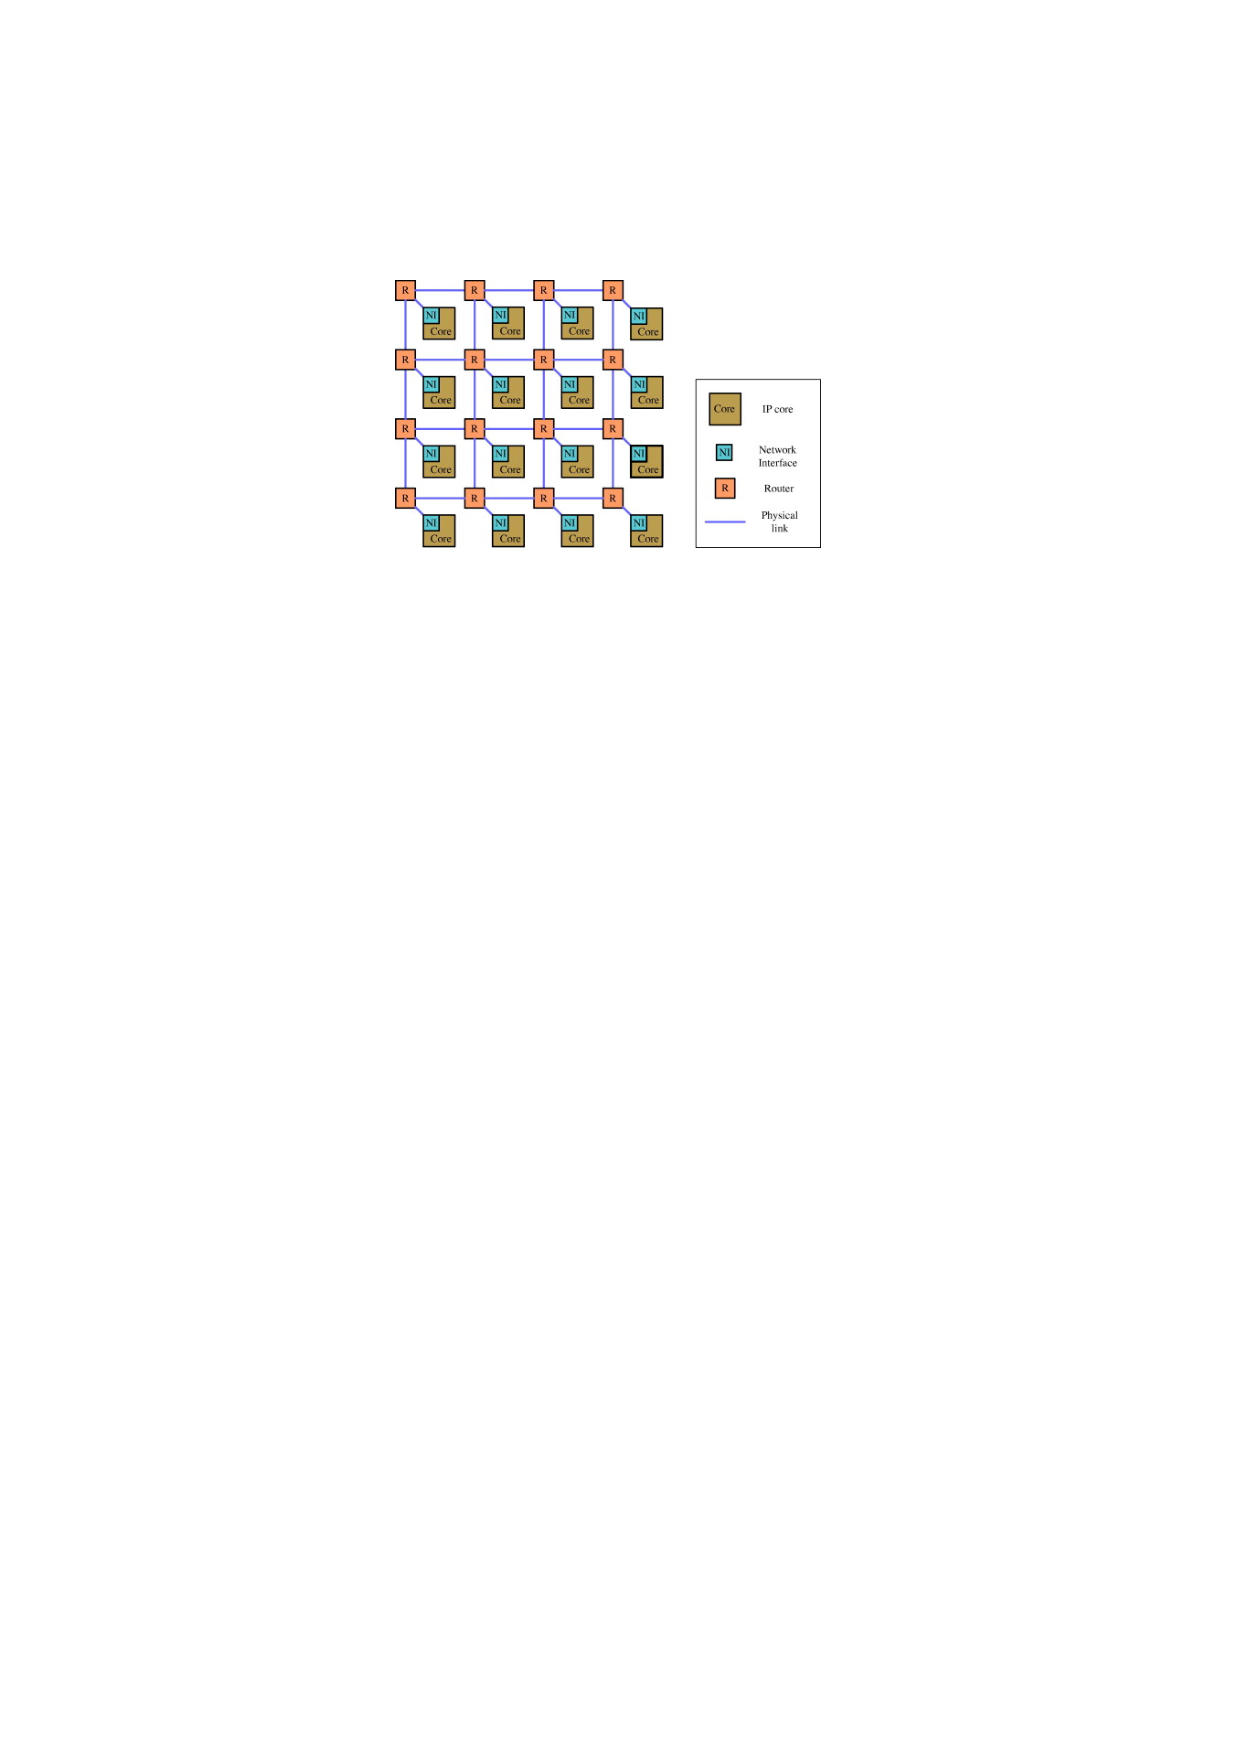
\includegraphics[width=0.5\textwidth]{Manycore}
    \caption{Net work on Manycore Processor}
    \label{fig:Manycore}
\end{figure}

众核处理器是一种通用处理器,这意味着他具有一定的灵活性,除了可以运用在神经网络运算上,还可以用在各种各样的领域,尤其是那些有高并行度要求的场景,例如 HPC。但如果仅针对深度神经网络的推理,通用处理器本身便会存在一些多余、不合适的设计。 

\subsection{GPU}

GPU 也可以看作是一种特殊的,针对向量运算的众核处理器。起初 GPU 被设计出来的目的是为了提高计算机对图像与视频的处理能力,但是当下,GPU 设备被广泛应用在深度学习应用的训练和推理加速中。并且对于 GPU 的调用,NVIDIA 还提供了软件支持,即 CUDA,方便了用户手动便携并行算子。

VOLTA 架构是 NVIDIA 推出的新一代的 GPU 设计架构,基于该架构的显卡被广泛运用在深度学习领域。其中,TESLA V100 是第一款被设计出来专门针对深度神经网络训练和推理的 GPU 设备(如图~\ref{fig:TESLA V100})。

\begin{figure}[!htbp]
    \centering
    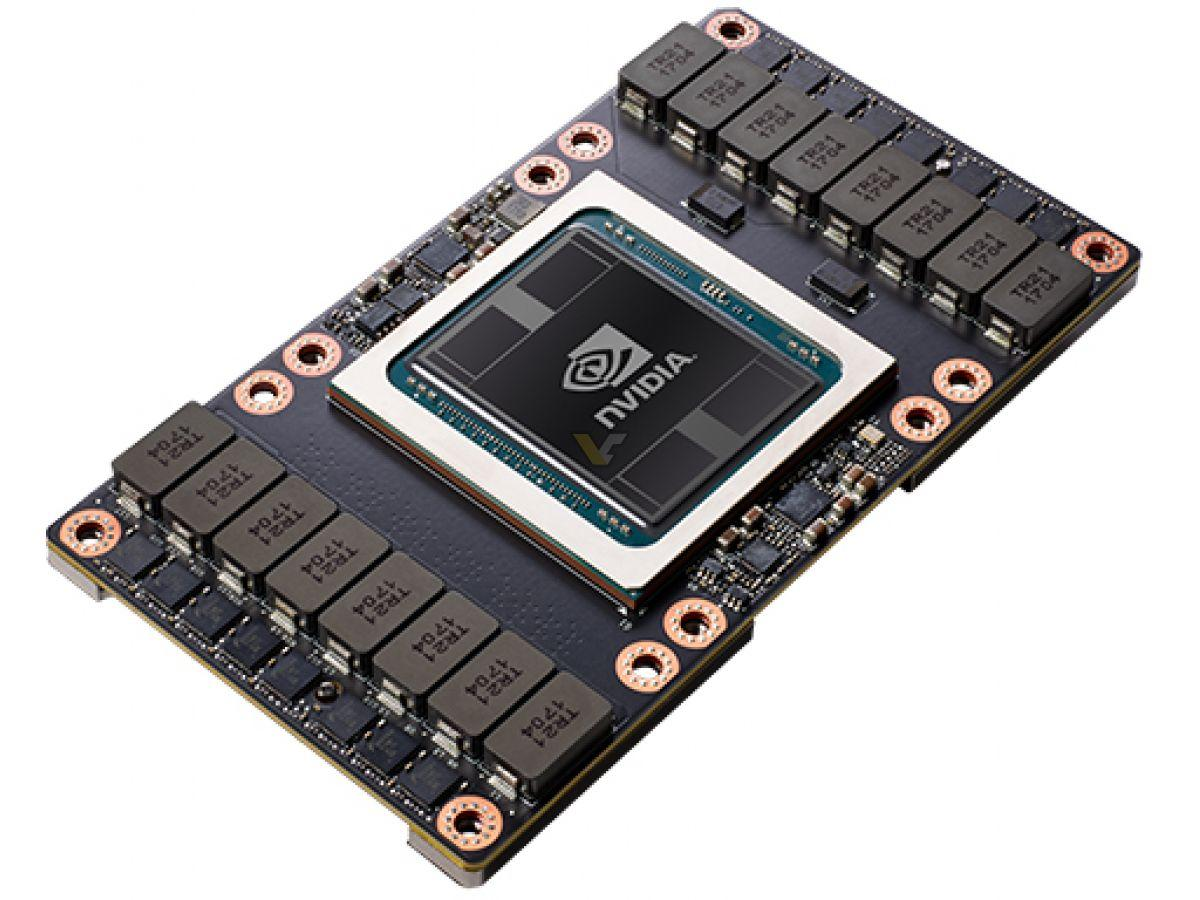
\includegraphics[width=0.5\textwidth]{TESLA V100.jpg}
    \caption{TESLA V100}
    \label{fig:TESLA V100}
\end{figure}

\subsection{Google TPU}

张量处理单元(Tensor Processing Unit)是 Google 牵头设计的一款为深度神经网络运算定制的 ASIC 器件,事实上其也取得了非常瞩目的性能,2015年发布的29nm工艺的 TPUv1 版本,能够运行在700Mhz的频率,但功率只有28W \textasciitilde 40W。

\subsection{DianNao 系列}

为了能够实现大规模深度学习网络的专用硬件执行。2014年,中国科学院计算技术研究所研究团队提出了 DianNao 架构。DianNao 这篇文章是率先探索机器学习加速设计的先驱文章之一,开创了专用处理器实现深度学习的先河。这篇文章在65nm工艺,0.98Ghz的频率,面积为3.02mm2的 ASIC 芯片上针对机器学习算法(DNN,CNN)实现了一个高性能的Diannao处理器架构,相比于128bit 2GHz的4发射SIMD处理器,达到了117.87x的加速比,21.08x能耗比。

\subsection{NVIDIA Deep Learning Accelerator}

NVDLA 是 NVIDIA 公司开源出来的深度学习加速器框架,其结构与 DianNao 类似。DianNao 系列芯片每个周期最多能够计算16个神经元,NVDLA 能够计算64个,而 TPU 则能够计算256个。

与前两个领域专用的硬件加速体系结构不同,NVDLA 完全开源,其不仅提供了 Verilog 硬件描述语言、CMOD 硬件仿真程序,还为硬件加速器设计了神经网络编译器与运行时,自上而下打通了硬件栈与软件栈,基本能够实现端到端的推理。虽然 NVDLA 自2018年以来已经没有人维护,但其系统设计思路仍然具有学习意义和指导意义。

因此,有关 NVDLA 的内容将在下一章节具体介绍。
